\documentclass[11pt,class=report,crop=false]{standalone}
\usepackage{exo7sv}

\begin{document}

%%%%%%%%%%%%%%%%%%%%%%%%%%%%%%%%%%%%%%%%%%%%%%%%%%%%%%%%%%%%%%%%%%%%%%
%%%%%%%%%%%%%%%%%%%%%%%%%%%%%%%%%%%%%%%%%%%%%%%%%%%%%%%%%%%%%%%%%%%%%%


%%%%%%%%%%%%%%%%%%%%%%%%%%%%%%%%%%%%%%%%%%%%%%%%%%%%%%%%%%%%
\section*{Problèmes d'optimisation}

\setcounterexo{6}

\exercice{}
\enonce
\begin{minipage}{0.59\textwidth}
    L'énergie dépensée par un poisson pour remonter une distance $d$ d'un courant de vitesse $u$ à la vitesse $v$ est donnée par
    $$
        E(v) = v^{3}\frac{d}{v-u}.
    $$
\end{minipage}
\begin{minipage}{0.4\textwidth}
\begin{tikzpicture}[x=1.00mm, y=1.00mm, scale=0.84]
    \clip (-2.00,-2.00) rectangle +(95.00,35);
    % la rivière
    \fill[blue!2]  (90.00,25.00) .. controls (88.68,20.80) and (84.15,18.54) .. (80.00,20.00) .. controls (76.40,21.27) and (73.93,25.36) .. (70.00,25.00) .. controls (66.15,24.65) and (63.94,19.91) .. (60.00,20.00) .. controls (56.09,20.09) and (53.94,25.02) .. (50.00,25.00) .. controls (46.07,24.98) and (43.93,20.02) .. (40.00,20.00) .. controls (36.06,19.98) and (33.91,24.91) .. (30.00,25.00) .. controls (26.06,25.09) and (23.85,20.35) .. (20.00,20.00) .. controls (16.07,19.64) and (13.60,23.73) .. (10.00,25.00) .. controls (5.85,26.46) and (1.32,24.20) .. (0.00,20.00) .. controls (0.00,15.00) and (0.00,5.00) .. (0.00,0.00) .. controls (22.50,0.00) and (67.50,0.00) .. (90.00,0.00) .. controls (90.00,6.25) and (90.00,18.75) .. (90.00,25.00);
    \draw[blue, thick] (0.00,20.00) .. controls (1.32,24.20) and (5.85,26.46) .. (10.00,25.00) .. controls (13.60,23.73) and (16.07,19.64) .. (20.00,20.00) .. controls (23.85,20.35) and (26.06,25.09) .. (30.00,25.00) .. controls (33.91,24.91) and (36.06,19.98) .. (40.00,20.00) .. controls (43.93,20.02) and (46.07,24.98) .. (50.00,25.00) .. controls (53.94,25.02) and (56.09,20.09) .. (60.00,20.00) .. controls (63.94,19.91) and (66.15,24.65) .. (70.00,25.00) .. controls (73.93,25.36) and (76.40,21.27) .. (80.00,20.00) .. controls (84.15,18.54) and (88.68,20.80) .. (90.00,25.00);

    % le poisson (version simple)
    % \filldraw[fill=white, draw=black] (10.00,15.00) .. controls (10.00,10.00) and (10.00,10.00) .. (10.00,5.00) .. controls (15.00,7.50) and (15.00,7.50) .. (20.00,10.00) .. controls (30.00,15.00) and (40.00,20.00) .. (45.00,10.00) .. controls (40.00,0.00) and (30.00,5.00) .. (20.00,10.00) .. controls (15.00,12.50) and (15.00,12.50) .. (10.00,15.00) -- cycle;

    % le poisson (version sophistiqué)
    \filldraw[fill=red!20, draw=black, yscale=-1] (0,0) svg "M 86.81,-12.16 C 86.05,-13.32 86.28,-13.46 86.04,-13.95 C 85.94,-14.15 85.75,-14.82 85.64,-15.45 C 85.38,-16.79 85.42,-16.86 86.65,-17.33 C 87.37,-17.60 87.42,-17.64 87.05,-17.72 C 82.68,-18.69 81.46,-19.02 79.66,-19.71 C 77.77,-20.44 78.73,-20.91 76.00,-18.14 C 74.84,-16.97 73.69,-15.90 73.45,-15.77 C 72.39,-15.15 71.24,-16.22 70.52,-16.52 C 70.20,-16.53 67.18,-19.52 66.84,-20.15 C 66.50,-20.74 66.02,-20.87 65.96,-21.18 C 65.90,-21.47 65.05,-22.26 64.98,-22.53 C 64.91,-22.80 64.07,-23.86 64.00,-24.13 C 63.92,-24.43 63.08,-25.20 63.01,-25.52 C 62.96,-25.76 62.07,-26.97 62.14,-27.23 C 62.27,-27.58 63.19,-27.89 65.60,-28.39 C 65.97,-28.47 65.96,-28.49 65.28,-29.23 C 63.40,-31.25 62.73,-31.87 62.28,-31.99 C 62.01,-32.05 60.40,-31.98 58.68,-31.83 C 54.70,-31.48 50.79,-31.47 49.65,-31.81 C 48.38,-32.19 47.82,-33.12 48.31,-34.03 C 48.40,-34.21 48.90,-34.55 49.41,-34.79 C 52.31,-36.15 55.55,-38.92 56.51,-40.87 C 56.88,-41.60 56.88,-41.73 56.88,-47.18 C 56.89,-53.52 56.91,-53.68 57.98,-53.77 C 58.50,-53.81 58.69,-53.72 59.35,-53.12 C 61.13,-51.47 62.16,-49.33 63.36,-44.81 C 64.07,-42.12 64.70,-40.70 65.64,-39.67 C 66.98,-38.21 69.79,-36.98 71.31,-37.18 C 72.12,-37.29 73.32,-37.89 73.32,-38.19
    C 73.30,-38.42 71.76,-39.41 71.03,-40.14 C 70.24,-40.94 70.56,-40.64 71.67,-43.01 C 72.41,-44.58 73.05,-45.00 73.15,-45.36 C 73.15,-45.53 73.46,-45.88 74.58,-47.00 C 75.29,-47.71 74.96,-47.80 75.57,-48.14 C 76.17,-48.47 76.39,-49.14 76.59,-49.22 C 77.28,-49.51 78.61,-50.98 80.41,-52.52 C 80.65,-52.73 81.13,-53.14 81.38,-53.35 C 81.68,-53.32 82.28,-53.27 82.58,-53.24 C 85.73,-52.96 89.11,-50.99 92.33,-47.58 C 92.71,-47.17 93.48,-46.36 93.87,-45.95 C 94.21,-45.95 94.90,-45.95 95.24,-45.95 C 102.61,-45.93 110.28,-43.82 116.07,-39.08 C 118.26,-37.29 120.93,-34.24 122.34,-31.93 C 122.91,-30.98 122.95,-30.79 122.67,-30.19 C 122.41,-29.63 123.08,-29.08 123.23,-28.59 C 123.44,-28.00 121.93,-26.32 119.67,-24.62 C 117.11,-22.70 113.56,-20.56 112.60,-20.36 C 111.88,-20.20 112.39,-20.11 111.04,-19.63 C 109.35,-19.02 109.22,-18.84 105.12,-18.16 C 104.11,-18.00 99.89,-17.26 98.25,-17.02 C 96.80,-16.80 95.51,-16.60 94.19,-16.43 C 93.30,-16.32 93.24,-16.23 92.92,-14.56 C 92.59,-12.80 92.06,-12.06 91.72,-13.34 C 91.59,-13.85 91.53,-13.99 90.38,-12.88 C 88.63,-11.20 87.66,-10.64 86.81,-12.16 Z";
    % l’oeil du poisson
    \begin{scope}
        \clip (39.00,12.00) circle (0.71mm);
        \filldraw[fill=white, draw=black] (39.00,12.00) circle (0.71mm);
        \filldraw[fill=black] (39.71,12.00) circle (0.71mm);
    \end{scope}

    % les vitesses
    \draw (0.00,0.00) -- (90.00,0.00);
    \draw[-latex] (47.00,10.00) -- (60.00,10.00) node[pos=0.5, above=1mm] {$v$};
    \draw[-latex] (80.00,15.00) -- (70.00,15.00);
    \draw[-latex] (80.00,10.00) -- (70.00,10.00);
    \draw[-latex] (80.00, 5.00) -- (70.00, 5.00);
    \node at (83,10) {$u$};

    % la distance parcouru
    \draw (20.00,22.00) -- (20.00,29.00);
    \draw (80.00,22.00) -- (80.00,29.00);
    \draw[latex-latex] (21.00,27.00) -- (79.00,27.00) node[pos=0.5, above=1mm] {$d$};

\end{tikzpicture}
\end{minipage}

    \begin{enumerate}
        \item Quel est le domaine de définition de cette fonction ?

        \item On se restreindra ici au domaine $]u,+\infty[$. Expliquer pourquoi.

        \item Étudier la fonction $E$ sur $]u,+\infty[$.

        \item En déduire la vitesse $v$ qui minimise l'énergie $E(v)$, puis calculer cette énergie minimale.
    \end{enumerate}    
\finenonce

\indication
Pour étudier la fonction il faut d'abord dériver la fonction $E(v)$ et étudier le signe de $E'(v)$.
\finindication

\correction

\video{RcW-KcNJfJ0}

\sauteligne
\begin{enumerate}
  \item Le domaine de définition est $\Rr \setminus \{u\}$, car pour $v=u$ il y aurait une division par zéro.

  \item Dans la pratique le poisson ne peut remonter le courant que si $v>u$, donc on étudie la fonction pour $v\in ]u,+\infty[$.

  \item 
$$E'(v) = d \left(\frac{v^3}{v-u}\right)'
= d \frac{3v^2(v-u)-v^3\cdot1}{(v-u)^2}
= d \frac{v^2(2v-3u)}{(v-u)^2}$$

Le signe de $E'$ ne dépend que du signe de $2v-3u$.
\begin{center}
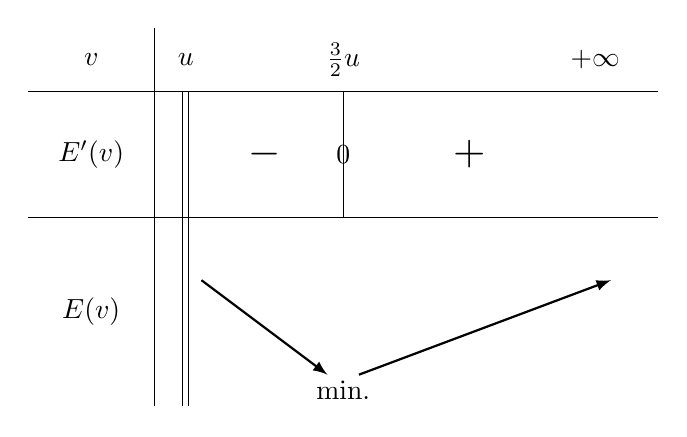
\begin{tikzpicture}[scale=0.8]

% Horizontales
% \draw(0,0) -- ++(10,0);
\draw(0,3) -- ++(10,0); 
\draw(0,5) -- ++(10,0); 

% Verticales
\draw(2,0) -- ++ (0,6);


% Première colonne
\node at (1,5.5) {$v$};
\node at (1,4) {$E'(v)$};
\node at (1,1.5) {$E(v)$};

% Autres colonnes
\node at (2.5,5.5) {$u$};
\draw(2.45,0) -- ++ (0,5);
\draw(2.55,0) -- ++ (0,5);

\node at (5,5.5) {$\frac32u$};
\node at (5,4) {$0$};
\draw(5,3) -- ++ (0,2);

\node at (9,5.5) {$+\infty$};

\node[scale=1.5] at (3.75,4) {$-$};
\node[scale=1.5] at (7,4) {$+$};

\draw[->,>=latex,thick](2.75,2)--++(2,-1.5);
\draw[->,>=latex,thick](5.25,0.5)--++(4,1.5);

\node[scale=1] at (5,0.25) {min.};
\end{tikzpicture}
\end{center}
  \item L'énergie est minimale pour $v=\frac32u$, c'est-à-dire lorsque le poisson nage à une vitesse valant $150\%$ de celle du courant.
\end{enumerate}
\fincorrection
\finexercice


\setcounterexo{9}


\exercice{}
\enonce
Dans une ruche, chaque alvéole a une forme de prisme hexagonal à fond rhombique dont la surface est donnée, pour une longueur de côté $s$ et une hauteur $h$, par 
\begin{equation*}
A(\theta) = 6sh - \frac{3}{2}s^{2}\frac{\cos(\theta)}{\sin(\theta)}+\frac{3\sqrt{3}}{2}s^{2}\frac{1}{\sin(\theta)}
\end{equation*}
où $\theta$ désigne l'angle au sommet du prisme.
\begin{center}
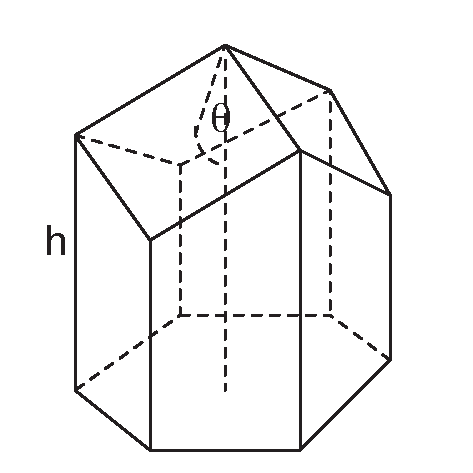
\includegraphics[width=6cm]{figures/abeille.pdf}
\end{center}
\begin{enumerate}
  \item Quelle est le domaine de d\'efinition de cette fonction ? 
  \item On se restreindra ici au domaine $]0,\pi[$. Expliquer pourquoi. 
  \item  Etudier la fonction $A$ sur $]0,\pi[$. 
  \item En déduire l'angle $\theta$ qui minimise la surface $A(\theta)$ d'une telle alvéole et déterminez, en fonction de $s$ et $h$, la surface correspondante.
\end{enumerate}
\textit{Dans la réalité, les alvéoles ont l'angle $\theta$ optimal à $\pm 2$ degrés près.}
\finenonce

\indication
On utilisera la fonction $\arccos : [-1; 1] \to [0; \pi]$ définie par $\arccos(x)=\theta \Leftrightarrow \cos(\theta)=x$.
De plus on a $\sin(\arccos(x)) = \sqrt{1-x^2}$ pour tout $x \in [0; 1]$.
\finindication

\correction

\video{UoLysyBdT7k}

\sauteligne
\begin{enumerate}
  \item L'expression définissant $A(\theta)$ est bien définie si et seulement si les dénominateurs sont non nuls, i.e. $\sin(\theta) \neq 0$.
  Or, $\sin(\theta)=0$ si et seulement $\theta=k\pi$ avec $k \in \mathbb{Z}$, ce que l'on peut réécrire $\theta \in \pi\mathbb{Z}$.
  On en déduit que le domaine de définition de $A$ est $\mathbb{R} \setminus \pi \mathbb{Z}$.
  \item L'angle au sommet du prisme doit avoir une mesure comprise dans l'intervalle $]0; \pi[$.
  On peut donc restreindre le domaine de $A$ à l'intervalle $]0; \pi[$ (ou à n'importe lequel des intervalles $]k; k+\pi[$ avec $k \in \mathbb{Z}$).
  \item On calcule la dérivée :
  \begin{align*}
  A'(\theta) &= -\frac32 s^2 \frac{\cos'(\theta)\sin(\theta)-\cos(\theta)\sin'(\theta)}{\sin(\theta)^2} + \frac{3\sqrt3}2 s^2 \frac{-\sin'(\theta)}{\sin(\theta)^2} \\
  &= -\frac32 s^2 \frac{-\sin(\theta)^2-\cos(\theta)^2}{\sin(\theta)^2} + \frac{3\sqrt3}2 s^2 \frac{-\cos(\theta)}{\sin(\theta)^2} \\
  &= -\frac32 s^2 \frac{-1}{\sin(\theta)^2} - \frac{3\sqrt3}2 s^2 \frac{\cos(\theta)}{\sin(\theta)^2} \\
  &= \frac32 s^2 \frac{1-\sqrt3\cos(\theta)}{\sin(\theta)^2}.
  \end{align*}
  On en déduit que :
  \begin{equation*}
  A'(\theta) = 0 \ \Leftrightarrow \ 1-\sqrt3\cos(\theta)=0 \ \Leftrightarrow \ \cos(\theta)=\frac1{\sqrt3} \ \Leftrightarrow \ \theta = \arccos(\frac1{\sqrt{3}}).
  \end{equation*}
   On en déduit le tableau de variation de $A$ :
  \begin{center}
    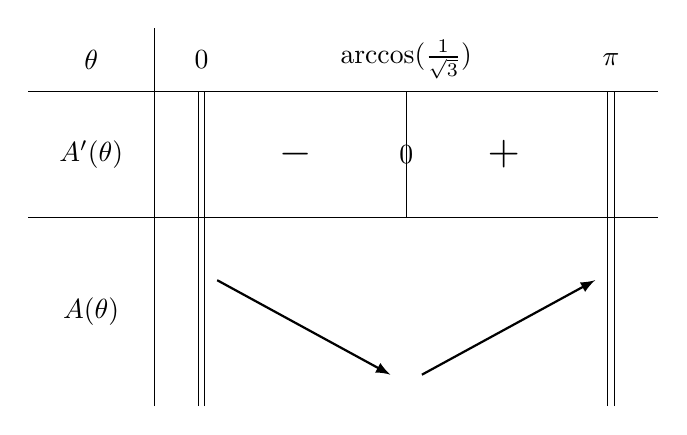
\begin{tikzpicture}[scale=0.8]
    % Horizontales
    % \draw(0,0) -- ++(10,0);
    \draw(0,3) -- ++(10,0); 
    \draw(0,5) -- ++(10,0); 
    
    % Verticales
    \draw(2,0) -- ++ (0,6);
    
    % Première colonne
    \node at (1,5.5) {$\theta$};
    \node at (1,4) {$A'(\theta)$};
    \node at (1,1.5) {$A(\theta)$};
    
    % Autres colonnes
    \node at (2.75,5.5) {$0$};
    \draw(2.70,0) -- ++ (0,5);
    \draw(2.80,0) -- ++ (0,5);
    
    \node at (6,5.5) {$\arccos(\frac1{\sqrt3})$};
    \node at (6,4) {$0$};
    \draw(6,3) -- ++ (0,2);
    
    \node at (9.25,5.5) {$\pi$};
    \draw(9.20,0) -- ++ (0,5);
    \draw(9.30,0) -- ++ (0,5);
    
    \node[scale=1.5] at (4.25,4) {$-$};
    \node[scale=1.5] at (7.55,4) {$+$};
    
    \draw[->,>=latex,thick](3,2)--++(2.75,-1.5);
    \draw[->,>=latex,thick](6.25,0.5)--++(2.75,1.5);
    \end{tikzpicture}
  \end{center}
  
  \item L'angle $\theta$ qui minimise la surface $A(\theta)$ est $\theta = \arccos(\frac1{\sqrt3}) \simeq 0,955$. Soit environ $54,7^\circ$.

  Pour la surface correspondante c'est un peu plus compliqué.
  On a :
  \begin{align*}
  \cos(\arccos(\frac1{\sqrt3})) &= \frac1{\sqrt3}, \\
  \sin(\arccos(\frac1{\sqrt3})) &= \sqrt{1-(\frac1{\sqrt3})^2} = \frac{\sqrt2}{\sqrt3}.
  \end{align*}
  La surface correspondante est donc :
  \begin{align*}
  A(\arccos(\frac1{\sqrt3})) &= 6sh - \frac32s^{2}\frac{\cos(\arccos(\frac1{\sqrt3}))}{\sin(\arccos(\frac1{\sqrt3}))}+\frac{3\sqrt{3}}{2}s^{2}\frac1{\sin(\arccos(\frac1{\sqrt3}))} \\
  &= 6sh - \frac32s^2\frac{\frac1{\sqrt3}}{\frac{\sqrt2}{\sqrt3}} + \frac{3\sqrt{3}}2s^{2}\frac1{\frac{\sqrt2}{\sqrt3}} \\
  &= 6sh - \frac3{2\sqrt2}s^2 + \frac9{2\sqrt2}s^2 \\
  &= 6sh + \frac3{\sqrt2}s^2.
  \end{align*}
\end{enumerate}
\fincorrection
\finexercice


\end{document}